\documentclass[12pt]{article}

\input{../Tex/header.tex}
%\geometry{twoside,bindingoffset = 2cm,left = 15mm, right = 15mm}
\onehalfspacing
\renewcommand{\bibname}{References}
% opening
\title{PhD Monitoring Report}
\author[1,2]{Samuel  Harrison}
\author[1]{\authorcr Supervisors: Dr Alex Lukyanov }
\author[2]{\authorcr Prof. D.T. Papageorgiou}

\affil[1]{ University of Reading}
\affil[2]{Imperial College London}
\date{\today}

\begin{document}
	\maketitle
	\section{PhD Motivation}
Deposition (e.g. stalagmites and stalactites) and dissolution (e.g. glaciers and icebergs) geomorphic patterns are fundamental in the environment,
and understanding the mechanisms underpinning their formation and evolution is central to paleo-reconstruction techniques used to
probe past climatological systems. Such problems pose numerous mathematical challenges including motion of free boundaries (wall-shape as well
as liquid-air interfaces), fluid-structure interactions and multiscale features in both space and time. The latter can pose particular challenges for
lab experiments (for instance features can form over time scales of hundreds of years) and we propose a complete theoretical approach
to quantify fundamental physical systems in order to compare with field observations.

\section{Work}
\subsection{Realistic Geometries}
Most of the research previously done on stalactites ignores the cylindrical geometry, treating the stalactite as a flat plate with a film on top \cite{short,camporeale_2017,doi:10.1098/rspa.2015.0031}. While this may give a good approximation for a smooth stalactite, the effects of the cylindrical geometry can not be ignored for when we model the stalactites to have crenulations. This is due to the radius of the stalactite and the wavelength of the crenulations being of similar order. Looking into research about flow down cylinders, many papers take the other extreme. That is making the radius of a comparable length to that of the fluid thickness\cite{ CRASTER_2006}. This method ignores some viscous terms and also some that appear due to the cylindrical geometry. A more realistic geometry for a stalactite can be found in a paper by Frenkel \cite{Frenkel_1992}. Here the radius of the cylinder is of the same order as the vertical length-scale which is much larger than that of the fluid thickness.
\subsection{Various Scalings}
In order to obtain a more realistic geometry for a stalactite I decided to try different scalings.
Here I started with the Navier Stokes equation in cylindrical coordinates, with no slip; no flux; tangential and normal stress balance; and the kinematic condition. These equations can be found in Appendix \ref{eqs}. I non-dimensionalised the equations using the film thickness as my length-scale and making it a gravity driven flow so that the velocity scales like $W\sim \frac{a_0^2 g}{\nu}$ where $a_0$ is the mean film thickness, $g$ the gravitational constant, and $\nu$ the kinematic viscosity. Then I changed $\hat{r}, \hat{z}$ to the new coordinates.
\begin{align}
\hat{r} = \frac{R}{\epsilon} + \frac{\eta(z)}{\varepsilon} + r \\
\hat{z} = \frac{z}{\delta}
\end{align}
where R is the radius of the stalactite, that for now is treated as a constant. $\eta$ is the shape of the crenulations. $\epsilon ,\varepsilon, \delta$ are small parameters to change the effective size of the radius, crenulation amplitude and crenulation wavelength. The wall is now at $r=0$ and the fluid-air interface is at $r = a$. In these schemes I also looked at how changing the magnitude of the Reynold's number $\Re = \frac{Ua_0}{\nu}$  and the Bond number $\Bo =\frac{\rho g a_0^2}{\gamma}$ would affect the flow. Changing the size of the Bond number introduces the surface tension into the flow through the pressure term. Changing the size of the Reynolds number can bring the inertia into the flow.
 Changing the size of $\epsilon$ allows the additional terms from the cylindrical Navier Stokes equations to be seen. Changing the size of $\varepsilon$ lets the wall have more of an effect on the flow. I then looked at several difference cases. For $\epsilon = \varepsilon = \delta$, the radius and crenulations are much larger than the fluid thickness. This case the $R$ can be absorbed into the $\eta$, meaning we don't necessarily have a clear radius. For  $\epsilon = \delta, \varepsilon = 1$ the crenulation amplitude are of similar order to the fluid thickness. This is the case for when the crenulations must first form on a stalactite, as stalactites start out as long thin ``soda straws".
 For $\epsilon =\delta = \varepsilon^2 $ the crenulations are much bigger than the fluid thickness however much smaller than the radius and wavelength. For $\epsilon = \varepsilon^2 = \delta^2$, we have the crenulations amplitude and wavelength of similar order, much larger than the fluid thickness however much smaller than the radius. For $\epsilon= \varepsilon^2, \delta = \varepsilon^{\frac{3}{2}}$  we have the fluid much thinner than the crenulation amplitude which is less than the crenulation wavelength which in turn is smaller than the radius of the stalactite. This case may best represent stalactites that occur naturally, but as all the features appear at different orders we must go to quite a high order to see all the effects. 
 \subsection{Steady States}
 Due to the difference in timescales for calcium deposition and the hydrodynamics, we can treat the fluid as steady \cite{short,PhysRevLett.108.238501}. Therefore when looking for the shape of the free surface I ignored the time derivative terms. The shape of the free surface could then be found by integrating the kinematic condition and equating terms that were found at the first 2 orders. This resulted in my fluid thickness being some function of the crenulations and their derivatives. Therefore I could make different crenulation shapes by looking at the Fourier series, to get a solution for the fluid thickness.

\begin{figure}[H]
	\caption{Example fluid thicknesses with a sinusoidal wall}	\begin{subfigure}{.33\linewidth}
	\centering
	\caption{Varying  the Surface Tension}
	\includegraphics[width =.9\linewidth]{varyBond}
\end{subfigure}	\begin{subfigure}{.33\linewidth}
	\centering
	\caption{Varying the Amplitude}
	\includegraphics[width =.9\linewidth]{varyA}
\end{subfigure}\begin{subfigure}{.33\linewidth}
	\centering
	\caption{Varying the Wavelength}
	\includegraphics[width =.9\linewidth]{varyL}
\end{subfigure}\end{figure}
These figures show the fluid thickness based on the dotted sinusoidal wall. They were made using the  $\epsilon= \varepsilon^2, \delta = \varepsilon^{\frac{3}{2}}$  case. They show that the fluid is thickest just before the maximum and thinnest just after the maximum. It can also be seen that by increasing the amplitude of the wall, increasing the Bond number, and decreasing the wavelength of the crenulations the fluid thickness increases.
\subsection{Chemistry of the Problem}
In order for the stalactite to grow, calcite must be deposited from the fluid onto the surface. The chemical reactions are described well in papers by Dreybrodt \cite{formation}. The concentrations of calcium and carbon dioxide form a pair of  reaction diffusion equations, with the boundary conditions being that there is no carbon dioxide flux and a calcium flux based on the rate of the reaction at the wall of the stalactite, and there is no calcium flux and a carbon dioxide flux which also depeneds on the rate of the reactions at the fluid-air interface.  The carbon dioxide also obeys Henry's law here. Since these equations depend on diffusion we must couple them with the fluid dynamics in order to determine how the wall shape changes due to the calcium deposited on it.
Several papers attempt to couple these equations \cite{short,camporeale_2017}. However at leading order the stalactite should just grow and the crenulations form due to higher order effects. In these papers some terms are not included which may also have an effect at this order. I tried coupling the various scalings that I used for the fluid dynamics with the reaction diffusion equation.




\subsection{Thin Film Equation approach}
Many papers that want to model a thin film come up with a thin film equation. I decided to try and incorporate the thin film down a cylinder from the paper with Frenkel \cite{Frenkel_1992} with the thin film over topography done by Tseluiko \cite{tseluiko_blyth_papageorgiou_2013}
This resulted in an equation for the film thickness.

\begin{align}
a_t + a_z a^2  +\epsilon\pdv{z}\left(\frac{a^4}{6R}+\frac{2}{15}\Re a^6a_z+ \frac{a^3}{3\Bo}\left(\frac{a_z+\eta_z}{R^2}+a_{zzz}+\eta_{zzz}\right)\right) + \epsilon\frac{\eta_z a^3}{3R}\label{walldyn}
\end{align}
where $a$ is the film thickness; $\epsilon$ is the ratio between the film thickness and the wavelength of the crenulation, a small parameter; $R$ is the ratio between the radius of the stalactites and wavelength of the crenulations; is the Reynold's number;  is the Bond number; $\eta$ is the shape of the crenulation.
Using this equation I wanted to see how changing the parameters effected the dynamics. I have made simulations using finite-difference methods to see how water will flow over topography based on this equation. I have simulated varying the amplitude and wavelength and shape of the crenulation, as well as varying the size of the radius, the Bond number and the Reynold's number. My results suggest that the fluid generally follows the topography of the surface however a small wave flows down the "stalactite" and gradually steepens. We are hoping to write a paper based off these findings.

\appendix
\section{Equations}
\subsection{Navier Stokes Equation in Cylindrical Coordinates \label{eqs}}

\begin{align}
\pdv{\tilde u}{\tilde r}+\frac{\tilde u}{\tilde r}+\pdv{\tilde w}{\tilde z}&=0\\
\pdv{\tilde u}{\tilde t}+\tilde u\pdv{\tilde u}{\tilde r}+\tilde w\pdv{\tilde u}{\tilde z}&=-\frac{1}{\rho}\pdv{\tilde p}{\tilde r}+\nu\left(\pdv[2]{\tilde u}{\tilde r}+\frac{1}{\tilde r}\pdv{\tilde u}{\tilde r}-\frac{1}{r^2}\tilde u+\pdv[2]{\tilde u}{\tilde z}\right)\\
\pdv{\tilde w}{\tilde t}+\tilde u\pdv{\tilde w}{\tilde r}+\tilde w\pdv{\tilde w}{\tilde z}&=-\frac{1}{\rho}\pdv{\tilde p}{\tilde z}+\nu\left(\pdv[2]{\tilde w}{\tilde r}+\frac{1}{\tilde r}\pdv{\tilde w}{\tilde r}+\pdv[2]{\tilde w}{\tilde z}\right) + g 
\end{align}
\subsection{Boundary Conditions}
\begin{align}
\tilde u=\pdv{\tilde R}{\tilde t},\;\tilde  w=0\quad\mathrm{on}\; \tilde r=\tilde R(\tilde z) 
\end{align}
\begin{align}
\tilde   u=\pdv{\tilde S}{\tilde t}+\tilde w\pdv{\tilde S}{\tilde z} \\
2\pdv{\tilde S}{\tilde z}\left(\pdv{\tilde u}{\tilde r}-\pdv{\tilde w}{\tilde z}\right)+\left(1-\left(\pdv{\tilde S}{\tilde z}\right)^2\right)\left(\pdv{\tilde u}{\tilde z}+\pdv{\tilde w}{\tilde r}\right)&=0\label{tangstress}\\
\tilde p\left(1+\left(\pdv{\tilde S}{\tilde z}\right)^2\right)-2\mu\left( \pdv{\tilde u}{\tilde r}-\pdv{\tilde S}{\tilde z}\left(\pdv{\tilde u}{\tilde z}+\pdv{\tilde w}{\tilde r}\right)+\left(\pdv{\tilde S}{\tilde z}\right)^2\pdv{\tilde w}{\tilde z}\right)&=\gamma\frac{\left(\frac{1}{\tilde S}\left(1+\left(\pdv{\tilde S}{\tilde z}\right)^2\right)-\pdv[2]{\tilde S}{\tilde z}\right)}{\left(1+\left(\pdv{\tilde S}{\tilde z}\right)^2\right)^{\frac{1}{2}}}\label{normstress}
\end{align}
\subsection{Chemical equations}
\begin{align}
\pdv{c_i}{t}+\vec{u}\cdot\grad c_i = P_i^{-1}\grad^2 c_i+r_i
\end{align} 
\begin{align}
\eval{\pdv{c_1}{r}}_{r=S} = 0,\quad \eval{\pdv{c_1}{r}}_{r=R} =A\tilde{f},\quad \eval{\pdv{c_2}{r}}_{r=S}=1,\quad \eval{\pdv{c_2}{r}}_{r=R}=0
\end{align}
where $c_i$ are the concentration, the subscript 1 refers to calcium and 2 refers to carbon dioxide. $P_i$ is the Peclet number, $r_i$ is a source or sink term relating to the net production. As calcium does not react with anything else in the system $r_1=0$. The net production of carbon dioxide is 
\begin{align}
r_2 = -k_1c_2+k_2(a_1c_1+a_2)
\end{align}
\begin{align}
\tilde{f} = -\kappa_1(\ce{H+})-\kappa_2(\ce{H2CO3^0 + CO2})-\kappa_3+\kappa_4(\ce{Ca^2+})(\ce{HCO3-})
\end{align}
\section{Example Stalactite}
\begin{figure}[H]
	\centering
	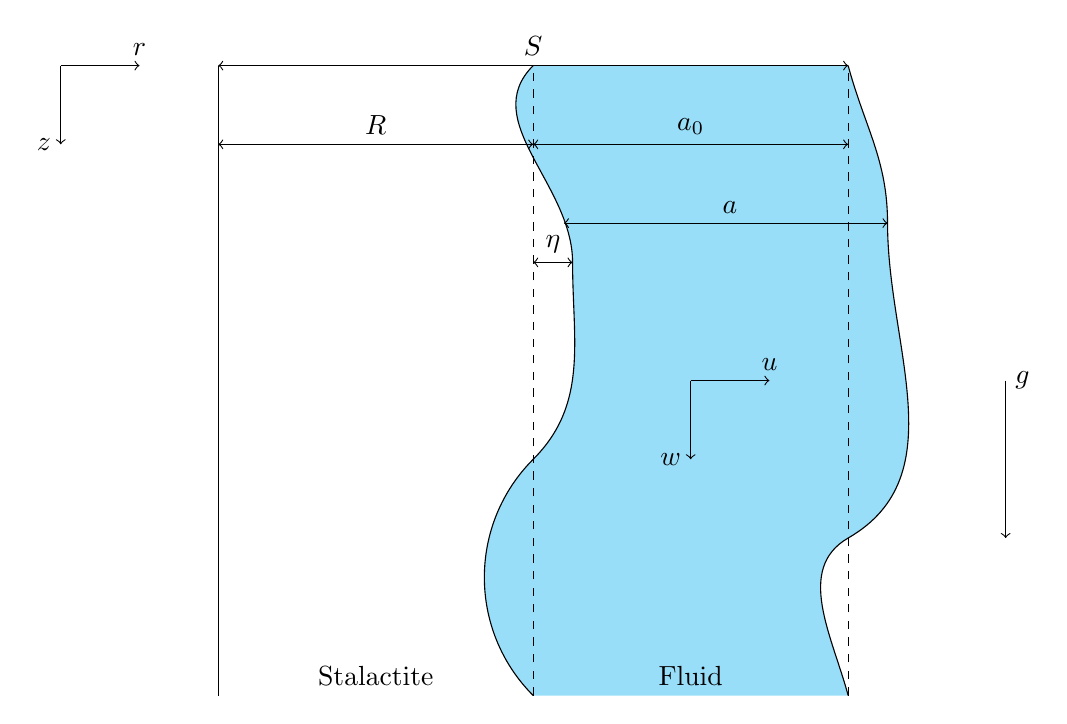
\begin{tikzpicture}
	\draw (0,0) -- (0,8);
	\fill[cyan!40!white] (4,0) to [out=135, in=-135] (4,3) to [out=45,in=-90]  (4.5,5.5) to [out=90,in=-135] (4,8) to (8,8) to [out=-75,in=90] (8.5,6) to [out=-90,in=30] (8,2) to [out=-150,in=105] (8,0) -- cycle;
	\draw[dashed](4,0) -- (4,8);
	\draw[dashed](8,0)--(8,8);
	\draw (4,0) to [out=135, in=-135] (4,3) to [out=45,in=-90]  (4.5,5.5) to [out=90,in=-135] (4,8);
	\draw (8,0) to [out=105, in=-150] (8,2) to [out=30,in=-90]  (8.5,6) to [out=90,in=-75] (8,8);
	\draw[<->](4,5.5)--(4.5,5.5);
	\node[above] at (4.25,5.5) {$\eta$};
	\draw[<->](4.39,6)--(8.5,6);
	\node[above] at (6.5,6) {$a$};
	\draw[<->] (0,7) --(4,7); 
	\node[above] at (2,7) {$R$};
	\draw[<->] (4,7) -- (8,7);
	\node[above] at (6,7) {$a_0$};
	\draw[->] (6,4) --(6,3);
	\node[ left] at (6,3) {$w$};
	\draw[->] (6,4) --(7,4);
	\node[above ] at (7,4) {$ u$};
	\draw[->] (10,4) --(10,2);
	\node[right] at (10,4) {$ g$};
	\draw[<->] (0,8)--(8,8);
	\node[above] at (4,8) {$ S$};
	\node[above] at (2,0) {Stalactite};
	\node[above] at (6,0) {Fluid};
	\draw[->] (-2,8) --(-2,7);
	\node[left] at (-2,7) {$ z$};
	\draw[->] (-2,8) --(-1,8);
	\node[above] at (-1,8) {$ r$};
	\end{tikzpicture}
	\caption{Stalactite with Crenulations\label{sta_cren}}
\end{figure}
\bibliographystyle{plain}
\bibliography{../MRES-Project/Report}
\end{document}